\documentclass[12pt]{article}
\usepackage{mathtools, amsfonts, bbm}
\usepackage{graphicx}
\usepackage{subcaption}

\title{Exercise 5}
\author{Shahaf \& Omri} 

\begin{document}
\maketitle

\section{1D}
\subsection{}
1. As we can see by the results we achieved ,The inductive bias assumption does hold , and indeed we can see that a somewhat cleaned image emerges before the noise is being reconstructed.

\begin{figure}[h!]
  \centering
  \begin{subfigure}[b]{0.4\linewidth}
    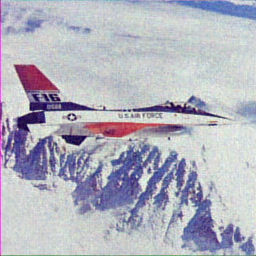
\includegraphics[width=\linewidth]{result1d.png}
    \caption{1000 epochs}
  \end{subfigure}
  \begin{subfigure}[b]{0.4\linewidth}
    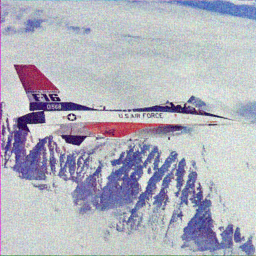
\includegraphics[width=\linewidth]{overfit1d.png}
    \caption{5000 epochs}
  \end{subfigure}
  \caption{A cleaner image emerges before noise is starting to be reconstructed}
  \label{fig:epoch_compare_1d}
\end{figure}

\subsection{}
We found using ADAM for optimization resulted in more pleasing results visually and faster convergence. In addition, using batch normalization was important for good results and a smoother image. We found learning rate of 1e-3 was a good fit, while 1e-5 was too slow, and bigger learning rates, such as 1e1, lead to bad results.
Increasing the number of filters also helped to achieve better results.
Our architecture is  5 convolution layers and 1 fully connected layer with 4 up-samples. We choose to use LeakyRelu as our activation function, and we used interpolation and then convolution in attempt to get less artifacts.

\begin{figure}[h!]
  \centering
  \begin{subfigure}[b]{0.4\linewidth}
    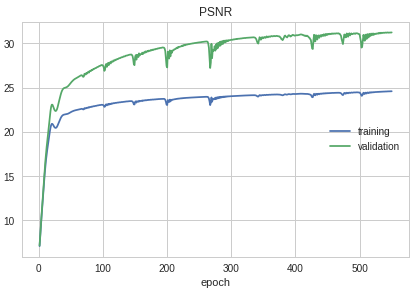
\includegraphics[width=\linewidth]{psnradam1d.png}
    \caption{using ADAM}
  \end{subfigure}
  \begin{subfigure}[b]{0.4\linewidth}
    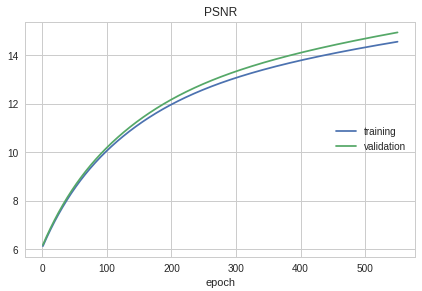
\includegraphics[width=\linewidth]{psnrsgd1d.png}
    \caption{using SGD}
  \end{subfigure}
  \caption{A major difference in results with using ADAM instead of SGD can be seen}
  \label{fig:grad_compare_1d}
\end{figure}

\begin{figure}[h!]
  \centering
  \begin{subfigure}[b]{0.4\linewidth}
    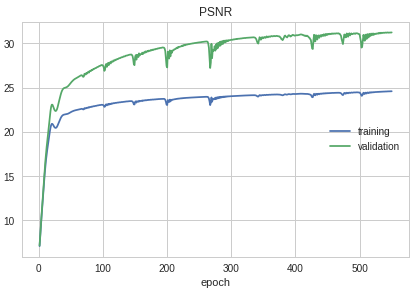
\includegraphics[width=\linewidth]{psnradam1d.png}
    \caption{Using L2}
  \end{subfigure}
  \begin{subfigure}[b]{0.4\linewidth}
    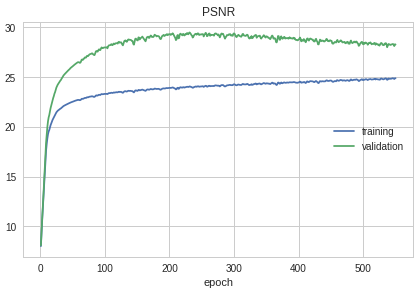
\includegraphics[width=\linewidth]{psnrL1in1d.png}
    \caption{Using L1}
  \end{subfigure}
  \caption{As we see, using L1 gets lower maximum, for the best results we used L2.}
  \label{fig:loss_compare_1d}
\end{figure}

\begin{figure}[h!]
  \centering
  \begin{subfigure}[b]{0.4\linewidth}
    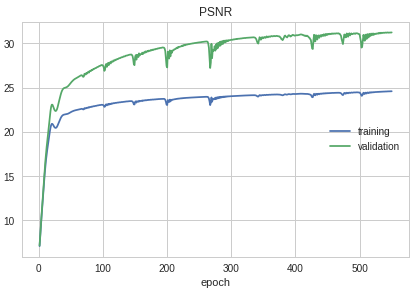
\includegraphics[width=\linewidth]{psnradam1d.png}
    \caption{using 1e-3 learning rate}
  \end{subfigure}
  \begin{subfigure}[b]{0.4\linewidth}
    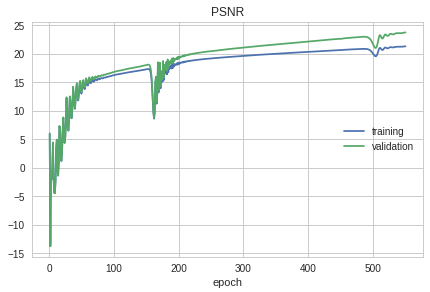
\includegraphics[width=\linewidth]{LR1e-1in1d.png}
    \caption{using 1e-1 learning rate}
  \end{subfigure}
  \caption{We see that a high learning rate will make it harder to converge , while a too small learning rate will cause convergence to be too slow.}
  \label{fig:learning_rate_1d}
\end{figure}

\subsection{PSNR}
First image 26.3 second 29.96 third 30.729 forth 30 the fifth 29.45 the six 28.14 the seven 30.36, the eight image 30.98 and the last has 30.3 ,  average of 29.58.

\subsection{}
we have \(6,468,835\) trainable parameters are in the model, \(1,376,780,288\) addition operations and \(1,376,772,096\) multiplication operations in our model. $\\ \\ \\ \\ \\ \\ \\ \\ \\ $

\section{2D}
\subsection{}
1. As we can see in \ref{fig:comparing_epoch_noise_2d}, the inductive bias assumption does hold , and indeed we can see that a somewhat cleaned image emerges before the noise is being reconstructed.

\begin{figure}[h]
  \centering
  \begin{subfigure}[b]{0.4\linewidth}
    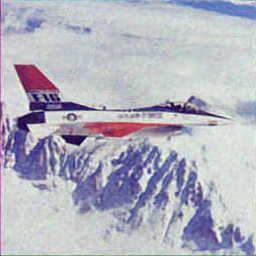
\includegraphics[width=\linewidth]{result2d.png}
    \caption{4000 epochs}
  \end{subfigure}
  \begin{subfigure}[b]{0.4\linewidth}
    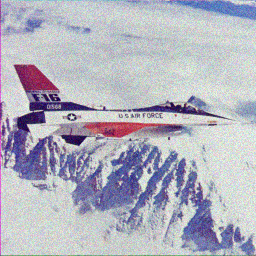
\includegraphics[width=\linewidth]{noisy2d.png}
    \caption{Image with the noise}
  \end{subfigure}
  \caption{As we can see a lot of the noise was indeed removed}
  \label{fig:comparing_epoch_noise_2d}
\end{figure}

\subsection{}
We found that using batch normalization was important for good results and a smoother image. 
Increasing the number of filters and parameters also helped achieving better results. We noticed that L2 is still better for us then using L1.
Our net is made of 9 convolution layers with 4 upsamples and 4 downsamples. We used at the beginning layers with convolution with strides (to downsample) and activation function and then we used layers with interpolation and then convolution, batch-norm and activation in attempt to get less artifacts.$\newline \newline$

\begin{figure}[h!]
  \centering
  \begin{subfigure}[b]{0.4\linewidth}
    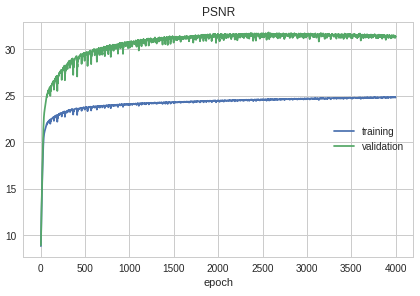
\includegraphics[width=\linewidth]{psnradam2d.png}
    \caption{Using 1e-3 learning rate}
  \end{subfigure}
  \begin{subfigure}[b]{0.4\linewidth}
    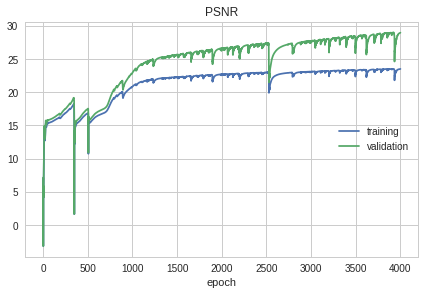
\includegraphics[width=\linewidth]{LR1e-1in2d.png}
    \caption{Using 1e-1 learning rate}
  \end{subfigure}
  \caption{Learning rate of 1e-3 performs better.)}
  \label{fig:learning_rate_2d}
\end{figure}

\subsection{PSNR}
First image 27.81 second 29.49 third 29.56 forth 27.95 the fifth 28.36 the six 27.72 the seven 28.56, the eight image 31.41 and the last has 28.61, in total we have average of 28.83.


\subsection{}
we have \(254,371\) trainable parameters are in the model, \(892,862,464\) addition operations and \(892,862,464\) multiplication operations in our model.

\section{2D with skip-connections}
\subsection{}
1. The architecture is the same as before but with "skip connections" , in which the information is propagated  through residual links. The network performance is similar to the 2D case.  The network does output a cleaner image in comparison to the noisy image but not completely smooth, as can be seen in Figure \ref{2ds results}. Indeed, it's easier for the network to output  a smoother, neutral image. The network does manage to over-fit the noise but very slowly. After 10,000 epochs the PSNR with respect to the noisy image, equalizes the PSNR with respect to clean image, As shown in Figure \ref{2ds overfit}. If we let the network train longer we will probably see the rend continuing albeit slowly.

\begin{figure}[h]
  \centering
  \begin{subfigure}[b]{0.3\linewidth}
    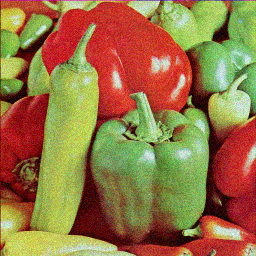
\includegraphics[width=\linewidth]{2ds_noisy.png}
    \caption{Noisy}
  \end{subfigure}
  \begin{subfigure}[b]{0.3\linewidth}
    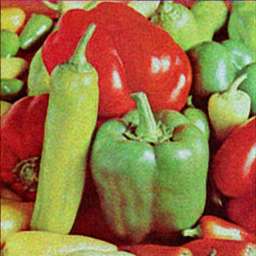
\includegraphics[width=\linewidth]{2ds_result.png}
    \caption{Result}
  \end{subfigure}
   \begin{subfigure}[b]{0.3\linewidth}
    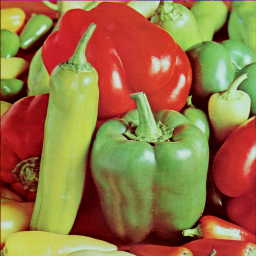
\includegraphics[width=\linewidth]{2ds_clean.png}
    \caption{Clean}
  \end{subfigure}
  \caption{2D with skip-connections after 1500 epochs}
  \label{2ds results}
\end{figure}

\begin{figure}[h]
	\centering
	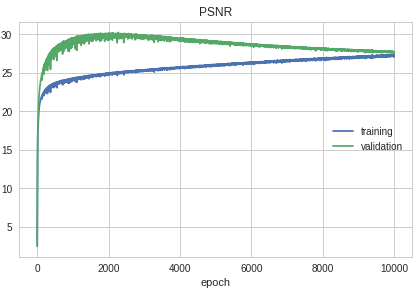
\includegraphics[width=0.8\linewidth]{2ds_overfit.png}
	\caption{PSNR for 10,000 epochs on image no. 5}
	\label{2ds overfit}
\end{figure}

\subsection{}
We Tried using half the amount of filters across all layers but we pretty much the same results except that with more filters PSNR grow faster, as can be seen in Figure \ref{resnet_vs_densnet}. We decided to keep using the same amount of filters.

\begin{figure}[h]
  \centering
  \begin{subfigure}[b]{0.4\linewidth}
    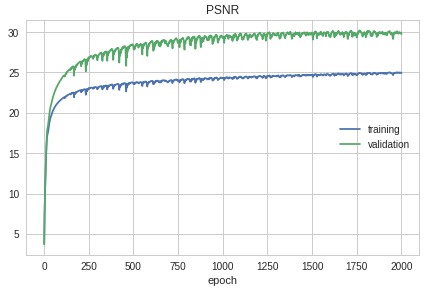
\includegraphics[width=\linewidth]{2dr.png}
    \caption{Vanilla architecture}
  \end{subfigure}
  \begin{subfigure}[b]{0.4\linewidth}
    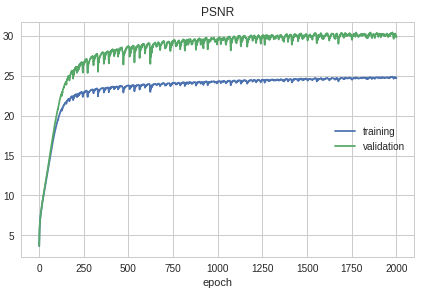
\includegraphics[width=\linewidth]{2ds_half_filters.png}
    \caption{Half the filters}
  \end{subfigure}
  \caption{PSNR using different amount of filters across all layers.}
  \label{resnet_vs_densnet}
\end{figure}

We also tried switching to a concatenation architecture. The PSNR for the residual links network was slightly better as shown in figure \ref{resnet vs densnet}.

\begin{figure}[h]
  \centering
  \begin{subfigure}[b]{0.4\linewidth}
    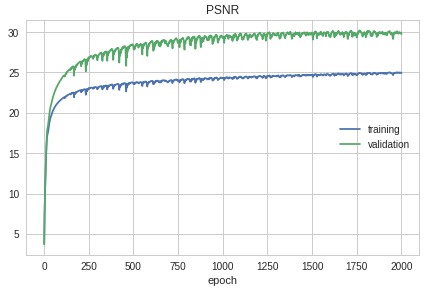
\includegraphics[width=\linewidth]{2dr.png}
    \caption{Residual Links}
  \end{subfigure}
  \begin{subfigure}[b]{0.4\linewidth}
    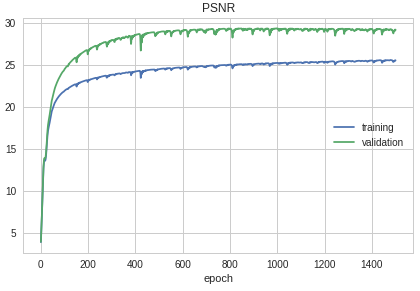
\includegraphics[width=\linewidth]{2ds_vanilla.png}
    \caption{With concatenation}
  \end{subfigure}
  \caption{PSNR - Residual links vs. Concatenation }
  \label{resnet vs densnet}
\end{figure}

\subsection{PSNR}
Results for residual links network:
PSNR by image: 26, 29.92, 30.61, 29.59, 30.05, 28.16, 30.1, 31.39, 30.1.
Total Average: 29.54.

\subsection{}
we have \(1866211\) trainable parameters are in the model, \(3093692416\) addition operations and \(3098542080\) multiplication operations in our model. $\\ \\ \\ \\ \\ \\ \\ \\ \\ $
\end{document}